\chapter{Quantum Relational Dynamics of Jaynes-Cummings Model
\label{chap5:RDQ_JCM_chap}}

In \refchap{chap:braun_briggs_jaynes}, we delved into the semi-classical approach to derive the Time-Dependent Schrödinger Equation (TDSE) governing the Jaynes-Cummings model. 
This method assumes a semiclassical (WKB-like) wave function for the field mode. However, 
this approach inherits the concept of ``time" as a purely classical parameter, thereby compromising its deeper and more fundamental nature.

In contrast, in \ref{chap:sebgem_Rel}, we presented a purely quantum framework to describe the dynamics of the general interacting system. Here, ``time" 
emerges as a symmetry parameter stemming from the principle of global invariance of the global energy 
eigenstate of total Hamiltonian.

This chapter explores the Jaynes-Cummings model from the perspective of Quantum Relational Dynamics. 
We aim to scrutinize the transition from a purely quantum system to semi-classical regimes, 
as previously discussed in \refchap{chap:braun_briggs_jaynes}, and to juxtapose the dynamics as 
characterized by the two distinct approaches. We demonstrate that, under appropriate limits
(consistent with the semi-classical treatment), the two approaches yield identical results. 
%Interestingly, the analysis also hints at the presence of a superselection rule.

We assume our Hamiltonian to be of the form

\begin{eqnarray}
        \label{eq:chap5_JCM_Hamiltonian}
        \oper{H} = \frac{\hbar \omega_0}{2} \oper{\sigma}_z + \hbar \omega \left(\oper{a}^\dagger \oper{a} + \frac{1}{2}\right) 
        + \hbar g \oper{\sigma}_x\left(\oper{a} + \oper{a}^\dagger\right). 
\end{eqnarray}


Under dipole-approximation and rotating-wave approximation 
[for details see~\refapp{app:chap3_appendix}], the Hamiltonian can be written as
\begin{equation}
        \label{eq:chap5_JCM_Hamiltonian_RWA}
        \oper{H} = \frac{\hbar \omega_0}{2} \oper{\sigma}_z + \hbar \omega \left(\oper{a}^\dagger \oper{a} + \frac{1}{2}\right) 
        + \hbar g \left(\oper{\sigma}_+ \oper{a} + \oper{\sigma}_- \oper{a}^\dagger\right).
\end{equation}

A specific scenario of this Hamiltonian, known as the "resonance case," becomes exactly solvable when \(\omega_0 = \omega\). 
This model is characterized by the Hamiltonian operator
\begin{equation}
        \label{eq:chap5_JCM_Hamiltonian_resonance}
        \oper{H} = \frac{\hbar\omega}{2} \oper{\sigma}_z + \hbar \omega \oper{a}^\dagger \oper{a}
        + \hbar g \left(\oper{\sigma}_+ \oper{a} + \oper{\sigma}_- \oper{a}^\dagger\right). 
\end{equation}
Here, it portrays the resonant interaction between two energy levels of an atom and a single mode within a cavity.
To investigate the dynamics of the JC-model, we initially aim to determine the evolution operator 
$U(t) = e^{-i t H/\hbar}$ through the diagonalization of $H$. If we achieve an eigenvalue decomposition 
$H = \sum_k a_k \lvert a_k \rangle \langle a_k \rvert$, it follows that:

\begin{equation}
U(t) = \sum_k e^{-i t a_k/\hbar} \lvert a_k \rangle \langle a_k \rvert
\end{equation}

Finding such an eigenvalue decomposition is not trivial, particularly in this context, 
given the infinite-dimensional nature of the underlying Hilbert space. However, the 
JC-Hamiltonian possesses a notably simple structure as it is block-diagonal with respect 
to the $\lvert \pm, n \rangle$-basis. The diagonalization of the JC-Hamiltonian in 
\refeq{eq:chap5_JCM_Hamiltonian_resonance} is given in \refapp{app:chap3_appendix}.
Once you block-diagonalize the Hamiltonian, the eigenvalues and eigenvectors of the JC-Hamiltonian are given by
\begin{equation}
        \label{eq:chap5_JCM_eigenvalues}
        E_{\pm, n} = \hbar \omega \left(n - \frac{1}{2}\right) \pm \hbar g \sqrt{n + 1},
\end{equation}
and the corresponding eigenvectors are
\begin{equation}
        \label{eq:chap5_JCM_eigenvectors}
        \lvert \pm, n \rangle = \frac{1}{\sqrt{2}} \left(\lvert g, n \rangle \pm \lvert e, n-1 \rangle\right).
\end{equation}


\begin{figure}[!h]
        \centering
        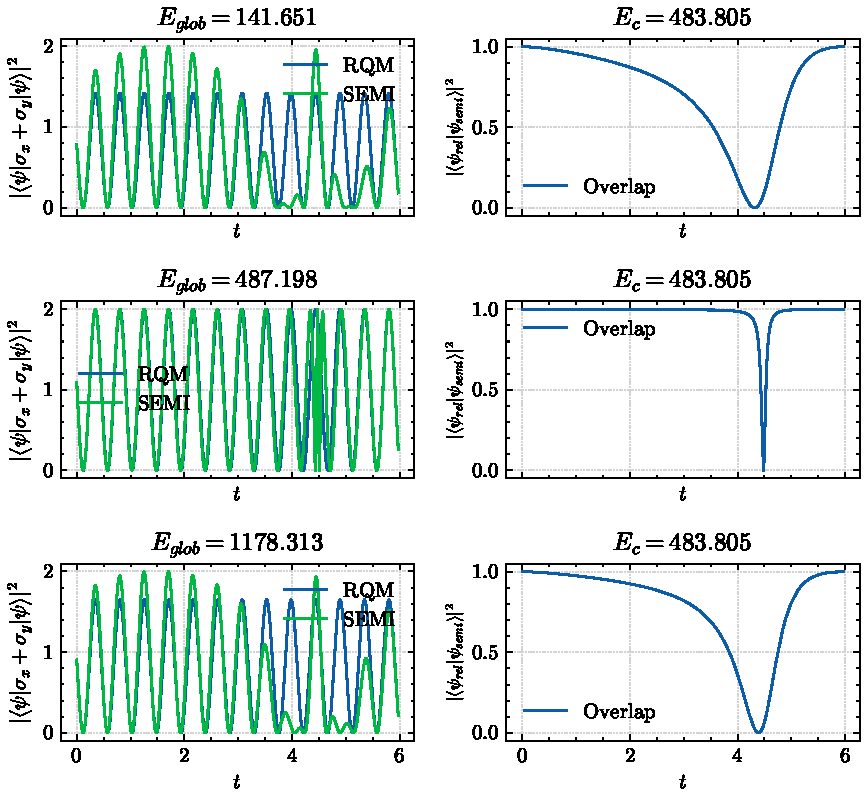
\includegraphics{chap5/semi_vs_quant.pdf}
        \caption[Expectation Value Comparison for Semi-Classical and
         Quantum Relational Dynamics]{Expectation Value Comparison 
         for Semi-Classical and Quantum Relational Dynamics. The $N_{\mathrm{cutoff}}=1000$ is taken for above calculations.}
        \label{fig:chap5_JCM_schematic}
\end{figure}
\begin{figure}[!h]
        \centering
        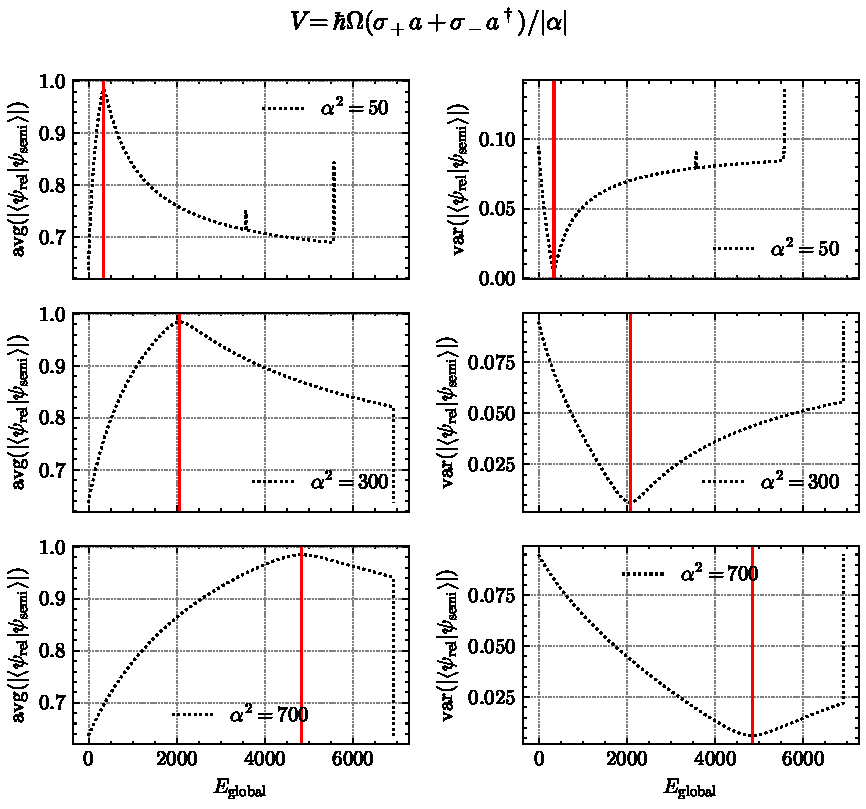
\includegraphics{chap5/overlap_average.pdf}
        \caption[Average $\abs*{\braket*{\psi_{rel}}{\psi_{semi}}}^2$ 
        (\& variance $\abs*{\braket*{\psi_{rel}}{\psi_{semi}}}^2$)
         v/s Global Eigen Energy]{The $N_{\mathrm{cutoff}}=1000$ is taken for above calculations.
         The plots shows the average $\abs*{\braket*{\psi_{rel}}{\psi_{semi}}}^2$ and 
         variance $\abs*{\braket*{\psi_{rel}}{\psi_{semi}}}^2$ over \(0, 2\pi\) v/s corresponding global eigen energy.
         An attempt to describe the dynamics of all eigenstates in a concise manner.}
        \label{fig:chap5_JCM_schematic_2}
\end{figure}